% Shock Engine research paper. Template filled by research/paper/build-paper.ts from the published
% research files: every figure in this document is read from them, none is typed by hand.
% Placeholders are upper-case names between double at-signs (values, tables and figures).
\documentclass[11pt,a4paper]{article}
\usepackage[T1]{fontenc}
\usepackage[utf8]{inputenc}
\usepackage{lmodern}
\usepackage[a4paper,margin=2.5cm,headheight=14pt]{geometry}
\usepackage{microtype}
\usepackage{amsmath,amssymb}
\usepackage{booktabs,tabularx,threeparttable,makecell}
\usepackage[table]{xcolor}
\usepackage{pgfplots}
\pgfplotsset{compat=1.18}
\usepgfplotslibrary{fillbetween}
\usepackage[font=small,labelfont=bf,margin=0pt]{caption}
\usepackage{enumitem}
\usepackage{fancyhdr}
\usepackage[authoryear,round]{natbib}
\usepackage[colorlinks=true,linkcolor=linkblue,citecolor=linkblue,urlcolor=linkblue,pdftitle={Shock Engine: Conditional Post-Shock Continuation in Bitcoin and Ether},pdfauthor={ShadowMarketPro Research}]{hyperref}

\definecolor{linkblue}{RGB}{20,70,140}
\definecolor{pfcol}{RGB}{0,140,110}
\definecolor{btccol}{RGB}{40,100,190}
\definecolor{ethcol}{RGB}{215,110,40}
\definecolor{bhcol}{RGB}{120,120,120}
\definecolor{negcol}{RGB}{190,50,50}

\setlist{itemsep=2pt,topsep=4pt}
\setlength{\parskip}{3pt}
\renewcommand{\arraystretch}{1.12}
\pagestyle{fancy}
\fancyhf{}
\fancyhead[L]{\small\itshape Shock Engine: conditional post-shock continuation}
\fancyhead[R]{\small\itshape ShadowMarketPro Research}
\fancyfoot[C]{\small\thepage}
\renewcommand{\headrulewidth}{0.3pt}

\newcommand{\SR}{\mathrm{SR}}
\newcommand{\E}{\mathbb{E}}
\newcommand{\1}{\mathbf{1}}

\begin{document}

\begin{titlepage}
\thispagestyle{empty}
\vspace*{1.2cm}
{\LARGE\bfseries Shock Engine: Conditional Post-Shock Continuation\\[4pt] in Bitcoin and Ether\par}
\vspace{10pt}
{\large Design, falsification and residual alpha of a systematic intraday strategy\par}
\vspace{18pt}
{\large ShadowMarketPro Research\par}
\vspace{4pt}
{\small Working paper v1.0 \textperiodcentered{} October 2026 \textperiodcentered{} specification E2 \textperiodcentered{} \texttt{shock-engine-2026.10}\par}
\vspace{22pt}
\begin{abstract}
\noindent We study a systematic strategy that trades the continuation of abnormal 15-minute price moves in Bitcoin (BTC) and Ether (ETH). A position is opened when a return that is extreme relative to its local volatility breaks the recent range and is confirmed by higher-timeframe structure, candle quality, participation and a price-impact filter; risk is managed with volatility-scaled exits. Shock Engine is defined by its specification E2, the reference version studied here, in which the short side is a \emph{conditional mirror} of the long side: short entries reproduce the long logic in the opposite direction and are admitted only when the daily trend regime is bearish. The rules were calibrated on Bitcoin and applied unchanged to Ether. Over 1~September 2018 to 30~September 2026, a 50/50 BTC/ETH portfolio shows a Sharpe ratio of 1.88, a compound annual growth rate of 61.6\% and a maximum drawdown of \ensuremath{-}19.1\% after transaction costs, against 0.78, 34.1\% and \ensuremath{-}76.9\% for buy-and-hold. Random-entry placebos, delayed entries, parameter neighbourhoods, cross-asset transfer, a Monte Carlo falsification battery for the short-entry condition and a regression on six standard trend-following strategies (residual alpha of 41.0\% a year, Newey--West $t=4.56$) do not explain the result away. The evidence is nonetheless in-sample: the Bitcoin rules were selected on data covering the period, and the short-entry condition was specified after the period had been studied. We report the failures (Solana, gold, TAO; a walk-forward Sharpe of 1.11) and pre-register a forward test.
\end{abstract}
\vspace{8pt}
\noindent{\small\textbf{Keywords:} cryptocurrency, intraday momentum, time-series momentum, jumps, regime conditioning, backtest overfitting, pre-registration, residual alpha.\\
\textbf{JEL:} G11, G12, G14, C12, C58.}

\vfill
\noindent{\footnotesize\textbf{Important.} All performance figures in this paper come from a historical simulation of fixed rules after modelled transaction costs. They are not live trading results. Simulated results have inherent limitations: they benefit from hindsight in the design of the rules and do not reflect the liquidity, slippage, funding and market impact of a real account. Past simulated performance does not predict future results. Nothing in this document is investment advice or an offer of any financial product or service.}
\end{titlepage}

\section{Introduction}

Cryptocurrency markets trade continuously, are dominated by a small number of liquid perpetual and spot venues, and move in bursts. A large share of daily variance arrives in a few intraday intervals, often after news, liquidations or the release of resting liquidity. Two competing views predict what happens next. Under \emph{underreaction}, information is incorporated gradually and a large move is followed by drift in the same direction \citep{HongStein1999}. Under \emph{overreaction} or liquidity provision, the move is partly a temporary price concession that reverts. Which view dominates is an empirical question, and the answer may depend on the state of the market.

This paper documents a rule-based strategy, \emph{Shock Engine}, built on the first view: it enters in the direction of an abnormal 15-minute move once the move has been qualified by a small set of filters, and exits through volatility-scaled risk management. Our contribution is less the rule itself than the way it is tested. We make five points.

\begin{enumerate}[label=(\roman*)]
\item The rules were set on Bitcoin and transferred \emph{without recalibration} to Ether, where they meet every pre-set criterion on two independent price feeds; they fail on Solana, gold and TAO, and we report these failures.
\item Random-entry placebos with identical exits and one-bar entry delays show that the edge lies in the timing of entries rather than in market drift or in the shape of the exits.
\item In specification E2, the reference version of Shock Engine, the short side is a \emph{conditional mirror} of the long side: short entries are allowed only in a bearish daily trend regime. Because this condition was specified after the sample had been studied, we subject it to three Monte Carlo falsification tests specified before they were run.
\item A regression of the daily returns on buy-and-hold and on six standard trend-following strategies leaves 79\% of the average return unexplained, with a Newey--West $t$-statistic of 4.56.
\item We pre-register a forward test of the short-entry condition with interim analyses, and run the strategy on Hyperliquid's test network so that its decisions are timestamped by a third party.
\end{enumerate}

The headline numbers are strong, which is precisely why they deserve suspicion. Throughout, we try to separate what the data can establish (the result is not a simple artefact of drift, exits, costs, a single parameter choice or a generic trend factor) from what it cannot (that the result will persist out of sample).

\section{Related literature}

\paragraph{Momentum and trend following.} Cross-sectional momentum in equities was documented by \citet{JegadeeshTitman1993}; \citet{MoskowitzOoiPedersen2012} show that an asset's own past return predicts its future return across futures markets (time-series momentum), and \citet{HurstOoiPedersen2017} extend the evidence over a century. Momentum payoffs are state dependent and can crash in rebounds after market declines \citep{DanielMoskowitz2016}, which motivates conditioning the short side on the state of the market rather than treating it as a symmetric copy of the long side. Simple trend rules based on moving averages and range breakouts were evaluated against bootstrap null models by \citet{BrockLakonishokLeBaron1992}; moving-average timing filters are popularised by \citet{Faber2007}.

\paragraph{Intraday dynamics and jumps.} \citet{GaoHanLiZhou2018} show that the first half-hour return of the S\&P~500 ETF predicts its last half-hour return, a form of intraday momentum linked to late-informed and hedging flows. Our shock statistic standardises a short-horizon return by an estimate of local volatility, in the spirit of the nonparametric jump test of \citet{LeeMykland2008}. Jumps cluster in time: self-exciting point processes \citep{Hawkes1971} capture this clustering and its propagation across markets \citep{AitSahaliaCachoDiazLaeven2015}, and one of our filters measures the local intensity of shocks. Scaling exposure and exits with volatility relates to the volatility-managed portfolios of \citet{MoreiraMuir2017}.

\paragraph{Cryptocurrency returns.} \citet{LiuTsyvinski2021} find that cryptocurrency returns load on crypto-specific factors, notably momentum and investor attention, rather than on traditional asset factors; \citet{LiuTsyvinskiWu2022} propose a three-factor model (market, size, momentum) for the cross-section of cryptocurrencies. Our strategy operates at a much shorter horizon, and Section~\ref{sec:alpha} measures how much of it a set of standard trend factors can span.

\paragraph{Overfitting and inference.} Searching many rules on one history inflates in-sample performance. \citet{White2000} and \citet{Hansen2005} propose reality checks for data snooping; \citet{BaileyLopezdePrado2014} deflate the Sharpe ratio for the number of trials and non-normality; \citet{BaileyEtAl2017} estimate the probability of backtest overfitting; \citet{HarveyLiuZhu2016} argue for a $t$-statistic hurdle of about 3 for new factors. We use heteroskedasticity- and autocorrelation-consistent standard errors \citep{NeweyWest1987}, block bootstraps \citep{Kunsch1989,PolitisRomano1994}, the Sharpe-ratio standard error of \citet{Lo2002}, and pre-registration with interim analyses in the tradition of clinical trials \citep{Haybittle1971,PetoEtAl1976,NosekEtAl2018}.

\section{Data and conventions}\label{sec:data}

Bitcoin is BTC/USD on Bitstamp and Ether is ETH/USDT on Binance spot, both in 15-minute bars timestamped at the open in UTC. After a warm-up period, Bitcoin is simulated from January 2017 and Ether from September 2018. An independent Ether feed (ETH/USD, Dukascopy) is used for replication. The common period of the portfolio is 1~September 2018 to 30~September 2026 (2{,}952 days, 8.1 years).

Daily returns are close-to-close on UTC days, the close of a day being the close of its last 15-minute bar. Annualisation uses $\sqrt{365.25}$ and a zero risk-free rate. Every order pays a commission of 0.045\% of notional, the base taker fee of the intended execution venue. Slippage and perpetual funding are \emph{not} included in the headline figures; Section~\ref{sec:frictions} adds them. Each market trades 100\% of its own capital, one position at a time, without leverage.

\section{The strategy}\label{sec:strategy}

We describe the logic of the rules and the mathematics of their building blocks. Thresholds, window lengths, timeframes and exit multiples are proprietary and are not disclosed; none of the tests below depends on knowing them. The specification is called E2: it is the reference version of Shock Engine, the one reported on the public website, run on the test network and covered by the pre-registration of Section~\ref{sec:forward}.

\subsection{Shock detection}

Let $P_t$ be the close of 15-minute bar $t$, $O_t,H_t,L_t$ its open, high and low, and $r_t=\ln(P_t/P_{t-1})$. Rolling estimates of the mean $\hat\mu_t$ and standard deviation $\hat\sigma_t$ of $r$ over a trailing window give the standardised return
\begin{equation}
z_t=\frac{r_t-\hat\mu_t}{\hat\sigma_t},\qquad S_t=\1\{|z_t|>\kappa\}.
\end{equation}
An up-shock ($S_t=1$, $r_t>0$) is directional when the close also breaks the range of the preceding bars, $P_t>\max_{t-h\le s<t}H_s$; a down-shock is the mirror image. The standardisation makes the trigger adaptive: the same absolute move is a shock in a calm market and noise in an agitated one, as in local-volatility jump tests \citep{LeeMykland2008}.

\subsection{Qualification}

A directional shock becomes an entry only if the following filters agree.
\begin{enumerate}[label=(\alph*)]
\item \emph{Structure.} Price is on the side of a higher-timeframe moving average that corresponds to the trade; long entries also require the average to be rising.
\item \emph{Candle quality.} The shock bar closes near its extreme with a small counter-direction wick, e.g.\ for a long $(H_t-\max(O_t,P_t))/(H_t-L_t)<\omega$, so that the move was not rejected within the bar.
\item \emph{Participation.} Volume is abnormal relative to its own recent distribution, $(V_t-\bar V_t)/s_{V,t}>\nu$.
\item \emph{Shock clustering.} The local intensity of shocks is estimated by an exponentially weighted average of past shock indicators,
\begin{equation}
\hat\lambda_t=(1-\eta)\,\hat\lambda_{t-1}+\eta\,S_t,
\end{equation}
and ranked against its own trailing distribution. Long entries require shocks to be clustering (a high percentile of $\hat\lambda_t$), the empirical signature of the self-exciting dynamics of jumps \citep{Hawkes1971,AitSahaliaCachoDiazLaeven2015}.
\item \emph{Volatility state.} The average true range, standardised against its own recent history, must lie below a regime-specific level, so that entries depend on the volatility state that precedes the shock.
\end{enumerate}
A short cooling-off period follows each trade.

\subsection{Volatility regimes}

Daily realised volatility over a short window is ranked against its own trailing one-year distribution. The market is \emph{calm} below the median and \emph{agitated} above. Each regime has its own parameter set (shock threshold, filters, exits, and the directions it may trade), and the active set is read from the last closed day, so that the rule never uses information from the current day.

\subsection{Exits and risk}

At entry the strategy records the average true range $A$. The initial stop is placed at $P_{\text{entry}}\mp m_s A$. Depending on the regime, part of the position may be taken off at $P_{\text{entry}}\pm m_p A$ and the remainder protected by a stop that trails the best price by $m_r A$. A position is also closed when price crosses back through a moving reference price, or when a qualified shock occurs in the opposite direction (flip exit). Each market holds at most one position, sized to its capital, with no pyramiding, no averaging down and no leverage.

\subsection{The short side: a conditional mirror}\label{sec:mirror}

Short entries reproduce the long logic in the opposite direction: a down-shock that breaks the recent low, closes near its low, occurs below the higher-timeframe average and is accompanied by abnormal volume. The long side carries additional qualification (rising structure and shock clustering), which reflects the asymmetry of crypto markets, whose long-run drift has been strongly positive.

In specification E2 the mirror is \emph{conditional} on the daily trend regime. With $D(t)$ the last UTC day closed before bar $t$, $P^{\mathrm{d}}_D$ the daily close, $\bar P^{(n)}_D$ a medium-term moving average of daily closes and $k$ a slope horizon in days,
\begin{equation}
T_t=\1\Big\{P^{\mathrm{d}}_{D(t)}<\bar P^{(n)}_{D(t)}\ \text{and}\ \bar P^{(n)}_{D(t)}<\bar P^{(n)}_{D(t)-k}\Big\},
\qquad
\text{Short}_t=\text{Mirror}_t\times T_t .
\end{equation}
Long entries, exits and the flip rule do not depend on $T_t$; the condition only decides whether a new short position may be opened. The economic motivation is the state dependence of momentum \citep{DanielMoskowitz2016}: selling a downside shock is a continuation trade in a falling market and a counter-trend trade in a rising one. Over the sample, 250 of the 1{,}311 trades are shorts.

\textbf{Disclosure.} An unconditional (symmetric) mirror was used while the strategy was developed. The trend condition that defines E2 was specified in October 2026, \emph{after} the period studied in this paper had been examined, so every historical figure in this paper is in-sample with respect to it. Section~\ref{sec:falsification} asks whether a condition of the same kind chosen at random would have done as well, and Section~\ref{sec:forward} tests it prospectively.

\subsection{Portfolio}

The portfolio allocates half of the capital to the Bitcoin strategy and half to the Ether strategy on the first day and never rebalances. Rebalancing monthly or weighting by risk changes the Sharpe ratio by at most 0.08 and is not part of the specification.

\section{Statistical framework}\label{sec:stats}

\paragraph{Performance.} With daily returns $r_d$, mean $\bar r$ and population standard deviation $s$,
\begin{equation}
\SR=\sqrt{365.25}\,\frac{\bar r}{s},\qquad
\text{Sortino}=\sqrt{365.25}\,\frac{\bar r}{\sqrt{\tfrac1N\sum_d \min(r_d,0)^2}},\qquad
\text{MDD}=\min_t\Big(\frac{V_t}{\max_{s\le t}V_s}-1\Big),
\end{equation}
and the Calmar ratio is CAGR$/|$MDD$|$. The standard error of an estimated annual Sharpe ratio over $T$ years is approximately \citep{Lo2002}
\begin{equation}\label{eq:lo}
\widehat{\mathrm{SE}}(\widehat\SR)\approx\sqrt{\frac{1+\tfrac12\SR^2}{T}} .
\end{equation}

\paragraph{Risk-normalised trade returns.} To compare trades across volatility regimes and assets, trade $i$ with profit $\pi_i$, equity at entry $E_i$ and entry day $d_i$ is scored as
\begin{equation}
R_i=\frac{\pi_i/E_i}{\sigma_{d_i}},
\end{equation}
where $\sigma_{d}$ is the standard deviation of the 30 daily log returns before day $d$. For a set of short trades, $\mathrm{EV}=\overline{R}$, and the regime contrast is
\begin{equation}
\Delta=\overline{R}_{\,T=1}-\overline{R}_{\,T=0}.
\end{equation}

\paragraph{Monte Carlo inference.} For a statistic $\theta$ and $N$ counterfactual draws $\theta^*_j$, the one-sided Monte Carlo $p$-value is
\begin{equation}
p=\frac{1+\#\{j:\theta^*_j\ge\theta\}}{1+N}.
\end{equation}

\paragraph{Residual alpha.} Daily strategy returns are regressed on benchmark returns,
\begin{equation}\label{eq:reg}
r_t=\alpha+\sum_{k=1}^{K}\beta_k f_{k,t}+\varepsilon_t,
\end{equation}
by ordinary least squares, with the Newey--West covariance
\begin{equation}
\hat V=(X^\top X)^{-1}\Big[\hat\Gamma_0+\sum_{l=1}^{L}\Big(1-\frac{l}{L+1}\Big)\big(\hat\Gamma_l+\hat\Gamma_l^\top\big)\Big](X^\top X)^{-1},
\qquad \hat\Gamma_l=\sum_{t=l+1}^{T}\hat\varepsilon_t\hat\varepsilon_{t-l}\,x_t x_{t-l}^\top,
\end{equation}
and lag $L=\lfloor4(T/100)^{2/9}\rfloor$. The residual information ratio is $\sqrt{365.25}\,\hat\alpha/\hat\sigma_\varepsilon$. A moving-block bootstrap draws calendar months with replacement, the same months for all series, so that cross-sectional dependence is preserved \citep{Kunsch1989}.

\section{Results}\label{sec:results}

\subsection{Headline performance}

Table~\ref{tab:headline} reports the two markets, the portfolio and a buy-and-hold benchmark built in the same way (half of the capital in each coin on the first day, no rebalancing, no costs). Figure~\ref{fig:equity} shows the equity curves on a logarithmic scale.

\begin{table}[tbp]
\centering\small\setlength{\tabcolsep}{5pt}
\begin{threeparttable}
\caption{Headline performance, 1~September 2018 to 30~September 2026}\label{tab:headline}
\begin{tabular}{lrrrr}
\toprule
 & Portfolio 50/50 & Bitcoin & Ether & Buy-and-hold \\
\midrule
Final value of 100 & 4{,}848 & 1{,}609 & 8{,}086 & 1{,}073 \\
CAGR & 61.6\% & 41.0\% & 72.2\% & 34.1\% \\
Annualised volatility & 27.6\% & 25.8\% & 34.3\% & 69.0\% \\
Sharpe ratio & 1.88 & 1.46 & 1.75 & 0.78 \\
Sortino ratio & 4.25 & 3.18 & 4.04 & -- \\
Maximum drawdown & \ensuremath{-}19.1\% & \ensuremath{-}22.3\% & \ensuremath{-}26.8\% & \ensuremath{-}76.9\% \\
Calmar ratio & 3.22 & 1.84 & 2.70 & 0.44 \\
Skewness of daily returns & 3.37 & 3.90 & 3.77 & -- \\
\midrule
Trades (long / short) & 1{,}311 (1{,}061 / 250) & 644 (508 / 136) & 667 (553 / 114) & -- \\
Trades per year & 162 & 80 & 83 & -- \\
Win rate & 31\% & 32\% & 30\% & -- \\
Average win / average loss & 4.37 & 4.00 & 4.68 & -- \\
Profit factor & 1.94 & 1.66 & 2.02 & -- \\
Median holding time (hours) & 4.0 & 3.5 & 4.5 & -- \\
Time in market & 26\% & 16\% & 18\% & 100\% \\
\bottomrule
\end{tabular}
\begin{tablenotes}[flushleft]\footnotesize
\item Historical simulation of specification E2 after modelled transaction costs; not live performance. Daily UTC close-to-close returns, annualised with $\sqrt{365.25}$, zero risk-free rate. Commission 0.045\% per order; no slippage, funding or leverage. Bitcoin and Ether columns are the two halves of the portfolio, each measured on its own capital. Buy-and-hold: half of the capital in each coin on 1~September 2018, no rebalancing, no costs. Win rate, payoff and profit factor are computed on closed trades; the portfolio column pools the trades of both markets.
\end{tablenotes}
\end{threeparttable}
\end{table}

\begin{figure}[tbp]
\centering
\begin{tikzpicture}
\begin{semilogyaxis}[width=\textwidth, axis lines*=left, grid=major, grid style={gray!20}, tick label style={font=\footnotesize}, label style={font=\footnotesize}, legend style={font=\footnotesize, draw=none, fill=white, fill opacity=0.85, text opacity=1}, legend cell align=left, height=7.2cm, xmin=2018.666, xmax=2026.745, xtick={2019,2020,2021,2022,2023,2024,2025,2026}, x tick label style={/pgf/number format/1000 sep={}}, xticklabel={\pgfmathprintnumber[fixed,precision=0,1000 sep={}]{\tick}}, ylabel={Value of 100 (log scale)}, legend pos=north west, log ticks with fixed point, ytick={25,50,100,250,500,1000,2500,5000}, yticklabel style={/pgf/number format/1000 sep={,}}]
\addplot[pfcol, very thick] table[x=x, y=pf] {data/equity.dat};
\addplot[btccol, thin] table[x=x, y=btc] {data/equity.dat};
\addplot[ethcol, thin] table[x=x, y=eth] {data/equity.dat};
\addplot[bhcol, thick, dashed] table[x=x, y=bh] {data/equity.dat};
\legend{Portfolio 50/50, Bitcoin, Ether, Buy-and-hold 50/50}
\end{semilogyaxis}
\end{tikzpicture}
\caption{Equity curves, 1~September 2018 to 30~September 2026, daily closes. Historical simulation after modelled transaction costs; buy-and-hold without costs.}\label{fig:equity}
\end{figure}

The return distribution is strongly right-skewed: the strategy is in the market 26\% of the time, wins 31\% of its trades, and its average winner is 4.4 times its average loser. The best 5\% of trades account for 136\% of the portfolio's log growth; without them the CAGR would be \ensuremath{-}17.2\%. This is the profile of a convex, trend-capturing strategy, and it implies that the result is sensitive to whether a few large moves are captured.

\subsection{Drawdowns and stability}

\begin{figure}[tbp]
\centering
\begin{tikzpicture}
\begin{axis}[width=\textwidth, axis lines*=left, grid=major, grid style={gray!20}, tick label style={font=\footnotesize}, label style={font=\footnotesize}, legend style={font=\footnotesize, draw=none, fill=white, fill opacity=0.85, text opacity=1}, legend cell align=left, height=5.2cm, xmin=2018.666, xmax=2026.745, xtick={2019,2020,2021,2022,2023,2024,2025,2026}, x tick label style={/pgf/number format/1000 sep={}}, xticklabel={\pgfmathprintnumber[fixed,precision=0,1000 sep={}]{\tick}}, ylabel={Drawdown}, ymax=0, yticklabel={\pgfmathparse{\tick*100}\pgfmathprintnumber[fixed,precision=0]{\pgfmathresult}\%}, legend pos=south west]
\addplot[bhcol, fill=bhcol!18, thin] table[x=x, y=bh] {data/drawdown.dat} \closedcycle;
\addplot[pfcol, fill=pfcol!35, thin] table[x=x, y=pf] {data/drawdown.dat} \closedcycle;
\legend{Buy-and-hold 50/50, Portfolio 50/50}
\end{axis}
\end{tikzpicture}
\caption{Drawdowns from the running peak, daily closes. Maximum: \ensuremath{-}19.1\% for the portfolio, \ensuremath{-}76.9\% for buy-and-hold.}\label{fig:dd}
\end{figure}

The deepest portfolio drawdown is \ensuremath{-}19.1\%, against \ensuremath{-}76.9\% for buy-and-hold (Figure~\ref{fig:dd}). Split in two halves, the portfolio Sharpe ratio is 2.03 (Sep.~2018--Sep.~2022) and 1.78 (Sep.~2022--Sep.~2026); the second half is weaker and the correlation between the two markets' strategy returns rises from 0.31 to 0.45. The rolling one-year Sharpe ratio (Figure~\ref{fig:rolling}) is positive in 100\% of windows and above one in 92\%, with a minimum of 0.28. A month-block bootstrap of 5{,}000 resampled histories gives a 90\% interval of 1.38 to 2.37 for the Sharpe ratio; a bootstrap resamples history and is not a forecast. Calendar-year results are in Table~\ref{tab:annual}.

\begin{figure}[tbp]
\centering
\begin{tikzpicture}
\begin{axis}[width=\textwidth, axis lines*=left, grid=major, grid style={gray!20}, tick label style={font=\footnotesize}, label style={font=\footnotesize}, legend style={font=\footnotesize, draw=none, fill=white, fill opacity=0.85, text opacity=1}, legend cell align=left, height=5cm, xmin=2018.666, xmax=2026.745, xtick={2019,2020,2021,2022,2023,2024,2025,2026}, x tick label style={/pgf/number format/1000 sep={}}, xticklabel={\pgfmathprintnumber[fixed,precision=0,1000 sep={}]{\tick}}, ylabel={Sharpe ratio}, ymin=0]
\addplot[black!45, dashed, domain=2010:2040, forget plot] {1};
\addplot[pfcol, thick] table[x=x, y=pf] {data/rolling.dat};
\end{axis}
\end{tikzpicture}
\caption{Rolling 365-day Sharpe ratio of the portfolio (2{,}588 windows). Positive in 100\% of windows, above one (dashed) in 92\%; median 1.76, minimum 0.28.}\label{fig:rolling}
\end{figure}

\begin{table}[tbp]
\centering\small
\begin{threeparttable}
\caption{Calendar-year returns}\label{tab:annual}
\begin{tabular}{lrrrrrr}
\toprule
Year & Bitcoin & Ether & Portfolio & Sharpe & Max.~drawdown & Buy-and-hold \\
\midrule
2018\tnote{a} & 18.8\% & 210.1\% & 114.5\% & 4.97 & \ensuremath{-}6.4\% & \ensuremath{-}50.3\% \\
2019 & 64.5\% & \ensuremath{-}14.3\% & 7.5\% & 0.43 & \ensuremath{-}15.1\% & 49.0\% \\
2020 & 15.5\% & 76.2\% & 50.5\% & 1.66 & \ensuremath{-}12.8\% & 355.8\% \\
2021 & 33.6\% & 65.8\% & 55.3\% & 1.84 & \ensuremath{-}9.3\% & 191.2\% \\
2022 & 46.1\% & 75.9\% & 67.6\% & 1.75 & \ensuremath{-}19.1\% & \ensuremath{-}66.4\% \\
2023 & 52.5\% & 12.9\% & 22.5\% & 1.09 & \ensuremath{-}7.3\% & 113.9\% \\
2024 & 114.0\% & 68.0\% & 81.9\% & 3.07 & \ensuremath{-}5.4\% & 78.1\% \\
2025 & \ensuremath{-}4.0\% & 99.1\% & 62.3\% & 1.91 & \ensuremath{-}10.5\% & \ensuremath{-}8.5\% \\
2026\tnote{a} & 16.7\% & 56.9\% & 48.4\% & 1.78 & \ensuremath{-}15.4\% & \ensuremath{-}6.8\% \\
\bottomrule
\end{tabular}
\begin{tablenotes}[flushleft]\footnotesize
\item \textsuperscript{a}\,Partial year (1~September 2018 to 31~December 2018; 1~January 2026 to 30~September 2026). Sharpe ratio and maximum drawdown are those of the portfolio within the year. Buy-and-hold is the 50/50 benchmark of Table~\ref{tab:headline}.
\end{tablenotes}
\end{threeparttable}
\end{table}

\subsection{Diversification}

Bitcoin and Ether prices are highly correlated (daily correlation 0.82), but the two strategies much less (0.36): each is out of the market most of the time and their trades rarely coincide. The portfolio Sharpe ratio exceeds that of either market alone. In seven named market stress episodes defined from spot prices only, the portfolio was positive in 6 of 7.

\subsection{Frictions}\label{sec:frictions}

\begin{table}[tbp]
\centering\small
\begin{threeparttable}
\caption{Transaction costs, slippage and funding (portfolio 50/50)}\label{tab:frictions}
\begin{tabular}{lrrr}
\toprule
Scenario & Sharpe & CAGR & Max.~drawdown \\
\midrule
\multicolumn{4}{l}{\textit{Commission per order}}\\
\quad 0.000\% & 2.14 & 74.0\% & \ensuremath{-}18.0\% \\
\quad 0.045\% (base case) & 1.88 & 61.6\% & \ensuremath{-}19.1\% \\
\quad 0.090\% & 1.61 & 50.2\% & \ensuremath{-}20.7\% \\
\multicolumn{4}{l}{\textit{Slippage per order, on top of the base commission}}\\
\quad 0.01\% & 1.82 & -- & -- \\
\quad 0.02\% & 1.76 & -- & -- \\
\quad 0.05\% & 1.58 & -- & -- \\
\multicolumn{4}{l}{\textit{Perpetual funding, on top of the base commission}}\\
\quad Historical perpetual funding (Binance) & 1.81 & 58.4\% & \ensuremath{-}19.2\% \\
\quad \quad with Hyperliquid funding from May 2023 & 1.80 & 57.6\% & \ensuremath{-}19.2\% \\
\quad Stress: shorts pay 0.01\% per 8 hours throughout & 1.86 & 60.7\% & \ensuremath{-}19.2\% \\
\bottomrule
\end{tabular}
\begin{tablenotes}[flushleft]\footnotesize
\item Funding is applied with its sign to long and short positions held across funding times; before 2020 a constant 0.01\% per 8 hours is assumed. Market impact and capacity are not modelled.
\end{tablenotes}
\end{threeparttable}
\end{table}

Turnover is high, about 157 times the capital a year, so costs matter. Doubling commissions, which is equivalent to adding 0.045\% of slippage on every fill, lowers the Sharpe ratio to 1.61. Historical perpetual funding, with the correct sign for long and short positions, lowers it to 1.81 (Table~\ref{tab:frictions}). Capacity and market impact are not modelled: the strategy enters precisely when liquidity is thinnest, which is the first thing a larger account would pay for.

\section{Robustness}\label{sec:robustness}

\subsection{Placebos, delays and transfer across markets}

For each market we fix pass/fail criteria before the result is seen: a positive event study of the signals and of shocks in the direction of the trend, a profit factor and a Sharpe ratio above preset levels, a rank above the 95th percentile of 200 random-entry runs that keep the exits identical, and a minimum share of the average trade retained when every entry is delayed by one bar. Table~\ref{tab:transfer} reports the result.

\begin{table}[tbp]
\centering\footnotesize\setlength{\tabcolsep}{3.6pt}
\begin{threeparttable}
\caption{Pre-set criteria by market, rules calibrated on Bitcoin only}\label{tab:transfer}
\begin{tabular}{llcrrrrrrl}
\toprule
Market & Feed & Period & Trades & Sharpe & CAGR & Max.~DD & Random & Delay & Verdict \\
\midrule
Bitcoin & Bitstamp & 2017--2026 & 774 & 1.56 & 42.9\% & \ensuremath{-}24.1\% & 100\% & 83\% & pass (in-sample) \\
Ether & Binance & 2018--2026 & 667 & 1.84 & 72.2\% & \ensuremath{-}29.5\% & 100\% & 94\% & pass \\
Ether & Dukascopy & 2019--2026 & 412 & 1.87 & 63.2\% & \ensuremath{-}26.4\% & 100\% & 72\% & pass \\
Solana & Binance & 2021--2026 & 398 & 0.35 & 6.1\% & \ensuremath{-}62.0\% & 87\% & 48\% & fail \\
Gold & Dukascopy & 2013--2026 & 663 & \ensuremath{-}0.07 & \ensuremath{-}0.5\% & \ensuremath{-}18.6\% & 100\% & n.m. & fail \\
TAO & Binance & 2024--2026 & 172 & \ensuremath{-}0.01 & \ensuremath{-}8.7\% & \ensuremath{-}50.4\% & 70\% & n.m. & fail \\
\bottomrule
\end{tabular}
\begin{tablenotes}[flushleft]\footnotesize
\item Each market is simulated over its full history with the Bitcoin rules unchanged. Sharpe ratios here are annualised from 15-minute returns and differ slightly from the daily figures of Table~\ref{tab:headline}. \emph{Random}: share of 200 random-entry runs with identical exits that the strategy beats (criterion: above 95\%). \emph{Delay}: share of the average trade kept when every entry is delayed by one bar (n.m.: not meaningful, average trade not positive). \emph{Verdict}: pass when the event study, profit factor, Sharpe, random-entry and delay criteria are all met; partial when the strategy criteria are met without the event study, or when only the Sharpe and random-entry criteria are met.
\end{tablenotes}
\end{threeparttable}
\end{table}

The random-entry placebo is the most informative test: with the exits held fixed, random entry times do much worse, so the edge is not a by-product of market drift or of the exit structure. Delaying every entry by one bar keeps most of the average trade, so the result does not depend on a perfect fill. Ether, never used for calibration, passes on two independent feeds. Solana, gold and TAO do not: the rules are not a universal law of markets, and we see no reason to hide it.

\subsection{Parameter neighbourhoods}

All parameters are perturbed together by up to $\pm5\%$, $\pm10\%$ and $\pm20\%$, with 300 random neighbours per level (Table~\ref{tab:neigh}). Every neighbour is profitable on both markets. On Bitcoin the chosen parameters sit at the top of their neighbourhood, as expected of rules selected on that data; on Ether they sit in the middle, a plateau rather than a peak.

\begin{table}[tbp]
\centering\small
\begin{threeparttable}
\caption{Parameter neighbourhoods: all parameters perturbed jointly, 300 neighbours per level}\label{tab:neigh}
\begin{tabular}{lrrrrrr}
\toprule
Market & Perturbation & Median Sharpe & P10--P90 & Chosen & Rank of chosen & Profitable \\
\midrule
Bitcoin & $\pm5\%$ & 1.45 & 1.35--1.53 & 1.56 & 95\% & 100\% \\
 & $\pm10\%$ & 1.38 & 1.24--1.51 & 1.56 & 97\% & 100\% \\
 & $\pm20\%$ & 1.32 & 1.17--1.47 & 1.56 & 99\% & 100\% \\
Ether & $\pm5\%$ & 1.85 & 1.70--2.01 & 1.84 & 47\% & 100\% \\
 & $\pm10\%$ & 1.86 & 1.62--2.02 & 1.84 & 45\% & 100\% \\
 & $\pm20\%$ & 1.77 & 1.55--1.97 & 1.84 & 68\% & 100\% \\
\bottomrule
\end{tabular}
\begin{tablenotes}[flushleft]\footnotesize
\item Sharpe ratios annualised from 15-minute returns over each market's full history. \emph{Rank of chosen}: percentile of the chosen parameters within their neighbourhood. \emph{Profitable}: share of neighbours with a positive total return.
\end{tablenotes}
\end{threeparttable}
\end{table}

\subsection{Walk-forward}

On Bitcoin, re-selecting the shock threshold, stop and trailing-stop settings of each regime every quarter on the previous 36 months only, choosing plateaus rather than isolated optima, over 28 windows from 2020 to 2026, gives a Sharpe ratio of 1.11 (15-minute returns), against 1.49 for the fixed settings over the same windows. The strategy remains profitable out of sample, but clearly below the fixed preset: part of the headline performance is a selection effect, and the forward test of Section~\ref{sec:forward} is the right place to measure it.

\section{Falsification of the short-entry condition}\label{sec:falsification}

The conditional mirror was introduced after the sample had been studied, so its in-sample improvement is not evidence. We pre-registered three tests asking whether the historical advantage is exceptional relative to counterfactuals with comparable properties. The condition itself is frozen; no parameter was changed after the results.

\paragraph{Test A: random selection.} Keep exactly as many of the original short trades as the condition keeps, chosen at random within each market and year, 50{,}000 times. The average risk-normalised return of the shorts actually kept ranks at the 96.8th percentile of the draws ($p=0.032$); the portfolio Sharpe ratio at the 94.5th percentile ($p=0.055$).

\paragraph{Test B: shifted regimes.} Shift the bearish periods circularly in time, keeping their persistence and their share of time, with a minimum shift of 180 days (2{,}593 shifts). The contrast $\Delta$ between shorts inside and outside the bearish regime is $0.436$ with the real dates, larger than with 99.6\% of the shifts ($p=0.005$ for the portfolio, 0.093 for Bitcoin and 0.001 for Ether).

\paragraph{Test C: synthetic markets.} Resample calendar blocks of 1, 3, 7, 14 and 30 days with replacement, the same blocks for both coins, rebuild synthetic 15-minute price paths, and recompute the engine, the regimes and the condition on each path (1,000 paths per block length). A generic effect of the condition would show up as a high probability of improvement on synthetic markets; an exceptional one as a historical improvement above the synthetic 95th percentile. Figure~\ref{fig:testc} shows the change in the average risk-normalised short return and Table~\ref{tab:testc} the details.

\begin{figure}[tbp]
\centering
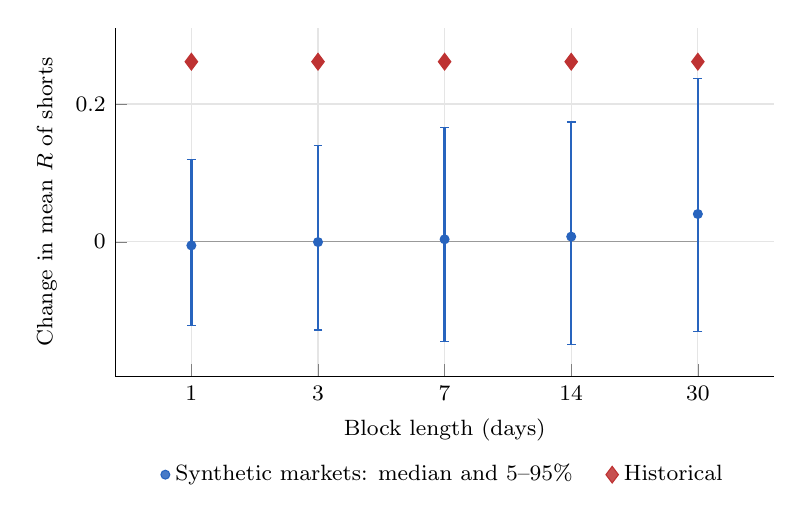
\begin{tikzpicture}
\begin{axis}[width=\textwidth, axis lines*=left, grid=major, grid style={gray!20}, tick label style={font=\footnotesize}, label style={font=\footnotesize}, legend style={font=\footnotesize, draw=none, fill=white, fill opacity=0.85, text opacity=1}, legend cell align=left, width=0.82\textwidth, height=6cm, symbolic x coords={1,3,7,14,30}, xtick=data, enlarge x limits=0.15, xlabel={Block length (days)}, ylabel={Change in mean $R$ of shorts}, ymax=0.31, yticklabel style={/pgf/number format/fixed}, legend style={at={(0.5,-0.22)}, anchor=north, /tikz/every even column/.append style={column sep=10pt}}, legend columns=2]
\addplot[black!40, forget plot] coordinates {(1,0) (30,0)};
\addplot[btccol, mark=*, mark size=1.6pt, only marks, error bars/.cd, y dir=both, y explicit, error bar style={btccol, line width=0.9pt}] coordinates {
  (1,-0.0053) += (0,0.1243) -= (0,0.1160)
  (3,-0.0004) += (0,0.1408) -= (0,0.1277)
  (7,0.0036) += (0,0.1627) -= (0,0.1480)
  (14,0.0075) += (0,0.1664) -= (0,0.1566)
  (30,0.0403) += (0,0.1972) -= (0,0.1704)
};
\addplot[negcol, mark=diamond*, mark size=3pt, only marks] coordinates {(1,0.2614) (3,0.2614) (7,0.2614) (14,0.2614) (30,0.2614)};
\legend{Synthetic markets: median and 5--95\%, Historical}
\end{axis}
\end{tikzpicture}
\caption{Test C. Change in the average risk-normalised return of short trades when the trend condition is applied, on 1{,}000 synthetic markets per block length and on the historical path. Historical percentile: 99.7\% ($L=1$), 99.6\% ($L=3$), 99.2\% ($L=7$), 99.4\% ($L=14$), 97.0\% ($L=30$).}\label{fig:testc}
\end{figure}

\begin{table}[tbp]
\centering\small
\begin{threeparttable}
\caption{Test C by block length: synthetic markets against the historical path}\label{tab:testc}
\begin{tabular}{rrrrrr}
\toprule
Block (days) & $P(\Delta\mathrm{EV}>0)$ & Synthetic P95 & Historical & Hist.~percentile & Sharpe gain, hist.~pct. \\
\midrule
1 & 0.47 & 0.119 & 0.261 & 99.7\% & 42.6\% \\
3 & 0.50 & 0.140 & 0.261 & 99.6\% & 52.6\% \\
7 & 0.51 & 0.166 & 0.261 & 99.2\% & 68.6\% \\
14 & 0.53 & 0.174 & 0.261 & 99.4\% & 74.8\% \\
30 & 0.66 & 0.238 & 0.261 & 97.0\% & 78.4\% \\
\bottomrule
\end{tabular}
\begin{tablenotes}[flushleft]\footnotesize
\item $\Delta\mathrm{EV}$: change in the mean risk-normalised return of shorts when the condition is applied (portfolio). \emph{Sharpe gain, hist.~pct.}: percentile of the historical change in portfolio Sharpe ratio among synthetic paths. The condition improved the maximum drawdown in 97\%, 94\%, 89\%, 87\%, 83\% of synthetic paths for $L=1,3,7,14,30$ days.
\end{tablenotes}
\end{threeparttable}
\end{table}

\paragraph{Reading.} On synthetic markets the condition improves the average short in only about half of the paths, so its benefit to the quality of shorts is not mechanical; the historical improvement exceeds the synthetic 95th percentile at every block length. By contrast, the gains in Sharpe ratio and drawdown are largely generic: removing shorts outside bearish regimes improves drawdowns in most synthetic paths as well. These tests use the same history that was studied before the condition was specified; they measure how unusual the result is, not how it will behave.

\section{Is it just trend following? Residual alpha}\label{sec:alpha}

A natural objection is that a strategy entering in the direction of large moves is a repackaged trend follower. We regress the portfolio's daily returns on buy-and-hold Bitcoin and Ether and on six standard trend strategies whose parameters were fixed before the study: time-series momentum over 30, 90 and 180 days, a 55/20-day breakout, a 20/100-day moving-average crossover and a 24h/12h breakout on 15-minute bars (Appendix~\ref{app:bench}). The benchmarks use the same bars and commissions, positions decided at the close and applied to the next period. The pre-set verdict required $\hat\alpha>0$, a Newey--West $t\ge3$ \citep{HarveyLiuZhu2016} and fewer than 1\% of bootstrap histories with $\hat\alpha\le0$. Table~\ref{tab:alpha} reports three nested models, Table~\ref{tab:bench} the benchmarks on their own and Figure~\ref{fig:betas} the loadings of the pre-set model.

\begin{table}[tbp]
\centering\small
\begin{threeparttable}
\caption{Residual alpha of the portfolio: regressions of daily returns on benchmark strategies}\label{tab:alpha}
\begin{tabular}{lrrr}
\toprule
 & M0 & M1 & M2 (pre-set) \\
\midrule
$\alpha$ (annualised) & \makecell[r]{49.6\%\\[-1pt]{\scriptsize(4.48)}} & \makecell[r]{40.3\%\\[-1pt]{\scriptsize(4.18)}} & \makecell[r]{41.0\%\\[-1pt]{\scriptsize(4.56)}} \\
\addlinespace
Buy-and-hold Bitcoin & \makecell[r]{\ensuremath{-}0.054\\[-1pt]{\scriptsize(\ensuremath{-}1.92)}} & \makecell[r]{\ensuremath{-}0.044\\[-1pt]{\scriptsize(\ensuremath{-}1.81)}} & \makecell[r]{\ensuremath{-}0.036\\[-1pt]{\scriptsize(\ensuremath{-}1.55)}} \\
Buy-and-hold Ether & \makecell[r]{0.077\\[-1pt]{\scriptsize(2.91)}} & \makecell[r]{0.073\\[-1pt]{\scriptsize(3.12)}} & \makecell[r]{0.077\\[-1pt]{\scriptsize(3.50)}} \\
TSMOM 30 days &  & \makecell[r]{0.089\\[-1pt]{\scriptsize(2.92)}} & \makecell[r]{0.066\\[-1pt]{\scriptsize(2.39)}} \\
TSMOM 90 days &  & \makecell[r]{0.046\\[-1pt]{\scriptsize(1.76)}} & \makecell[r]{0.051\\[-1pt]{\scriptsize(1.46)}} \\
TSMOM 180 days &  & \makecell[r]{\ensuremath{-}0.047\\[-1pt]{\scriptsize(\ensuremath{-}1.60)}} & \makecell[r]{\ensuremath{-}0.063\\[-1pt]{\scriptsize(\ensuremath{-}2.18)}} \\
Breakout 55/20 days &  & \makecell[r]{0.078\\[-1pt]{\scriptsize(1.94)}} & \makecell[r]{0.051\\[-1pt]{\scriptsize(1.35)}} \\
Moving averages 20/100 days &  & \makecell[r]{\ensuremath{-}0.001\\[-1pt]{\scriptsize(\ensuremath{-}0.04)}} & \makecell[r]{0.031\\[-1pt]{\scriptsize(1.09)}} \\
Intraday breakout 24h/12h &  &  & \makecell[r]{0.162\\[-1pt]{\scriptsize(5.89)}} \\
\midrule
$R^2$ & 0.022 & 0.152 & 0.266 \\
Residual information ratio & 1.82 & 1.59 & 1.74 \\
Share of mean return unexplained & 96\% & 78\% & 79\% \\
Bootstrap $P(\alpha\le0)$ & -- & -- & 0.0000 \\
Bootstrap 90\% interval of $\alpha$ & -- & -- & 26.1\% to 55.8\% \\
\bottomrule
\end{tabular}
\begin{tablenotes}[flushleft]\footnotesize
\item 2{,}952 daily observations, 1~September 2018 to 30~September 2026. Newey--West $t$-statistics in parentheses (lag 8). M0: buy-and-hold only; M1: adds five daily trend strategies; M2: adds the intraday breakout. Bootstrap: 5{,}000 resamples of 97 calendar months, the same months for all series. Pre-set verdict for M2: $\alpha>0$, $t\ge3$ and $P(\alpha\le0)<0.01$.
\end{tablenotes}
\end{threeparttable}
\end{table}

\begin{table}[tbp]
\centering\small
\begin{threeparttable}
\caption{Benchmark strategies on their own, and sensitivity of the residual alpha}\label{tab:bench}
\begin{tabular}{lrrrr}
\toprule
Benchmark (50/50, after costs) & Sharpe & CAGR & Max.~drawdown & Corr.~with SE \\
\midrule
Buy-and-hold 50/50 & 0.82 & 37.7\% & \ensuremath{-}76.3\% & 0.11 \\
TSMOM 30 days & 0.96 & 50.9\% & \ensuremath{-}52.2\% & 0.33 \\
TSMOM 90 days & 0.45 & 7.9\% & \ensuremath{-}90.6\% & 0.21 \\
TSMOM 180 days & 0.36 & 2.7\% & \ensuremath{-}89.3\% & 0.09 \\
Breakout 55/20 days & 0.84 & 35.4\% & \ensuremath{-}59.1\% & 0.33 \\
Moving averages 20/100 days & 0.64 & 22.6\% & \ensuremath{-}69.9\% & 0.21 \\
Intraday breakout 24h/12h & 0.02 & \ensuremath{-}14.8\% & \ensuremath{-}88.6\% & 0.38 \\
Shock Engine portfolio & 1.88 & 61.6\% & \ensuremath{-}19.1\% & 1.00 \\
\midrule
\textit{Sensitivity of M2} & $\alpha$ & $t$ & $R^2$ & IR \\
\midrule
19 trend strategies (full grid) & 40.7\% & 4.73 & 0.343 & 1.82 \\
First half (Sep.~2018--Sep.~2022) & 46.2\% & 3.21 & 0.219 & 1.75 \\
Second half (Sep.~2022--Sep.~2026) & 38.1\% & 3.90 & 0.423 & 2.01 \\
Weekly returns & 42.6\% & 4.37 & 0.346 & 1.66 \\
Benchmarks without costs & 36.0\% & 4.17 & 0.266 & 1.52 \\
\bottomrule
\end{tabular}
\begin{tablenotes}[flushleft]\footnotesize
\item Benchmarks average the two markets with daily rebalancing and pay the same commission as Shock Engine (0.045\% per order); buy-and-hold carries no costs. Corr.~with SE: correlation of daily returns with the Shock Engine portfolio. Definitions in Appendix~\ref{app:bench}.
\end{tablenotes}
\end{threeparttable}
\end{table}

\begin{figure}[tbp]
\centering
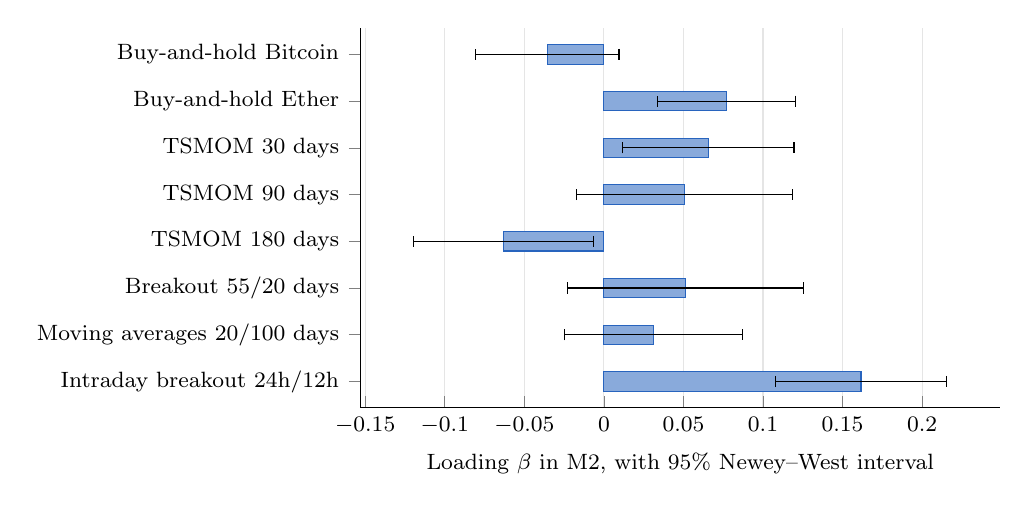
\begin{tikzpicture}
\begin{axis}[width=\textwidth, axis lines*=left, grid=major, grid style={gray!20}, tick label style={font=\footnotesize}, label style={font=\footnotesize}, legend style={font=\footnotesize, draw=none, fill=white, fill opacity=0.85, text opacity=1}, legend cell align=left, width=0.8\textwidth, height=6.4cm, xbar, bar width=7pt, y dir=reverse, symbolic y coords={Buy-and-hold Bitcoin,Buy-and-hold Ether,TSMOM 30 days,TSMOM 90 days,TSMOM 180 days,Breakout 55/20 days,Moving averages 20/100 days,Intraday breakout 24h/12h}, ytick=data, xlabel={Loading $\beta$ in M2, with 95\% Newey--West interval}, enlarge y limits=0.08, xmajorgrids, ymajorgrids=false, scaled x ticks=false, xticklabel style={/pgf/number format/fixed, /pgf/number format/precision=2}]
\addplot[fill=btccol!55, draw=btccol, error bars/.cd, x dir=both, x explicit, error bar style={black}] coordinates {
  (-0.0357,Buy-and-hold Bitcoin) +- (0.0452,0)
  (0.0771,Buy-and-hold Ether) +- (0.0432,0)
  (0.0656,TSMOM 30 days) +- (0.0539,0)
  (0.0506,TSMOM 90 days) +- (0.0680,0)
  (-0.0629,TSMOM 180 days) +- (0.0565,0)
  (0.0514,Breakout 55/20 days) +- (0.0743,0)
  (0.0311,Moving averages 20/100 days) +- (0.0561,0)
  (0.1616,Intraday breakout 24h/12h) +- (0.0538,0)
};
\end{axis}
\end{tikzpicture}
\caption{Factor loadings of the portfolio in the pre-set model M2. The largest loading is on the intraday breakout ($t=5.89$), which loses money on its own after costs.}\label{fig:betas}
\end{figure}

The residual alpha is 41.0\% a year with $t=4.56$; no bootstrap history out of 5{,}000 produced $\hat\alpha\le0$, and the 90\% interval is 26.1\% to 55.8\%. The factors explain $R^2=0.27$ of the daily variance and leave 79\% of the average return unexplained. The largest loading is on the intraday breakout, which shares part of the timing of the strategy but loses money on its own after costs. Using 19 trend strategies at once, which deliberately favours the benchmarks, leaves the conclusion unchanged ($t=4.73$). The verdict is ``residual alpha demonstrated, in-sample'': simple trend strategies do not reproduce the historical result. The regression cannot tell whether the alpha will persist.

\section{Forward validation and live deployment}\label{sec:forward}

\paragraph{Pre-registered forward test.} The hypothesis $H_1:\ \E[R\mid T=1]>\E[R\mid T=0]$ for short signals is tested prospectively from 12~October 2026, with the definition, statistic, thresholds and stopping date committed before the first observation. Interim analyses occur when 25, 50 and 75 shorts have closed in the bearish regime, each at $p<0.001$; the final analysis occurs when both groups reach 100 closed shorts, at $p<0.047$, and no later than 1~October 2031, for a total type-I error of at most 0.05 \citep{Haybittle1971,PetoEtAl1976}. With roughly 162 trades a year across both markets, few of them shorts, the test will take years rather than months.

\paragraph{Why live Sharpe ratios take time.} By Equation~\eqref{eq:lo}, a strategy with a true Sharpe ratio of 1.5 observed for one year has a standard error of about 1.46: a single year of live trading cannot distinguish it from zero. What a first year can establish is \emph{implementation fidelity}: that the live system takes the same decisions as the simulation on the same bars, at a measurable execution cost.

\paragraph{Deployment.} The live engine shares its decision code with the backtester and is tested for decision-by-decision parity. Since 9~October 2026 it runs the public specification on Hyperliquid's test network, where every order is publicly timestamped by the exchange; testnet funds are fictitious and its market differs from the real one, so these results check mechanics, not performance.

\section{Limitations}

\begin{itemize}
\item \textbf{Selection.} The Bitcoin rules were selected on 2017--2026 data, which contains the whole portfolio period; Ether is a transfer across markets, not across time. The walk-forward Sharpe ratio (1.11) is clearly below the fixed preset.
\item \textbf{Post-hoc condition.} The short-entry condition was specified after the period had been studied; Section~\ref{sec:falsification} measures how unusual its benefit is but does not make it out-of-sample.
\item \textbf{Frictions.} Slippage and funding are excluded from the headline figures. Capacity and market impact are not modelled, and the strategy trades when order books are thinnest.
\item \textbf{Right tail.} A small number of large trades drive the long-run growth; missing a few of them in live trading would change the outcome materially.
\item \textbf{Venues.} Data venues (Bitstamp, Binance spot) differ from the intended execution venue (Hyperliquid perpetuals) in prices, fees, funding and stop mechanics.
\item \textbf{Multiple testing.} Many tests are reported. Their criteria were fixed in advance and failures are reported, but the overall research process still involved choices that no single test accounts for.
\end{itemize}

\section{Conclusion}

Shock Engine trades the continuation of qualified 15-minute shocks in Bitcoin and Ether, with a short side that mirrors the long side only in bearish daily regimes. On eight years of data the 50/50 portfolio delivers a Sharpe ratio of 1.88 with a maximum drawdown of \ensuremath{-}19.1\%, survives placebo, delay, cost, parameter and cross-asset tests, and is not spanned by standard trend strategies. The same evidence is in-sample, depends on a convex right tail, and excludes capacity. The decisive tests are the pre-registered forward analysis and a live track record, both under way and reported as they arrive, whatever they show.

\clearpage
\appendix
\section{Benchmark strategies}\label{app:bench}

For each market, a position $q_t\in\{-1,0,1\}$ is decided at the close of period $t$ with information up to $t$ and earns $q_t\,(P_{t+1}/P_t-1)-c\,|q_t-q_{t-1}|$ with $c=0.045\%$. Portfolio factors average the two markets with daily rebalancing; buy-and-hold Bitcoin and Ether enter separately.
\begin{itemize}
\item \textbf{Time-series momentum} TSMOM$(L)$: $q_t=\operatorname{sign}(P_t/P_{t-L}-1)$, $L\in\{30,90,180\}$ days.
\item \textbf{Breakout} (55/20 days): from flat, long if $P_t>\max_{t-55\le s<t}P_s$ and short if $P_t<\min_{t-55\le s<t}P_s$; a long exits when $P_t<\min_{t-20\le s<t}P_s$ and a short when $P_t>\max_{t-20\le s<t}P_s$.
\item \textbf{Moving averages} (20/100 days): $q_t=+1$ if $\mathrm{EMA}_{20}(t)>\mathrm{EMA}_{100}(t)$, $-1$ otherwise.
\item \textbf{Intraday breakout} (15-minute bars): the breakout rule with 96-bar entry and 48-bar exit windows (24 and 12 hours).
\end{itemize}
Long-only versions are not added: with positions $\pm1$ their returns are, up to costs, the average of the long/short version and buy-and-hold, already in the span of the regressors.

\section{Synthetic markets (Test C)}

Calendar blocks of $L$ days are drawn with replacement from the full history, the same blocks for both coins. Within a block, 15-minute bars are rescaled so that the synthetic path is continuous at block boundaries; volumes are normalised by their trailing mean; the price grid follows a fixed rule. The engine, the volatility regimes and the trend condition are recomputed from scratch on each path. On the identity path the construction reproduces the original strategy exactly (identical regimes and equity bar by bar), which validates the pipeline.

\section{Reproducibility}

Every number in this paper is produced by versioned code from versioned data and read from the published research files (research version \texttt{shock-engine-2026.10}, code commit \texttt{0aac2d8}, parameter hash \texttt{c6ac30464bce}); the portfolio pipeline runs 40 consistency checks, all passing. Pre-registration documents were committed before the corresponding computations. Data files, daily returns and the full numerical report are available at \url{https://www.shadowmarketpro.com/research}.

\clearpage
\begin{thebibliography}{99}
\setlength{\itemsep}{2pt}\small

\bibitem[A\"it-Sahalia et~al.(2015)]{AitSahaliaCachoDiazLaeven2015} A\"it-Sahalia, Y., Cacho-Diaz, J., and Laeven, R.~J.~A. (2015). Modeling financial contagion using mutually exciting jump processes. \emph{Journal of Financial Economics}, 117(3), 585--606.

\bibitem[Bailey et~al.(2017)]{BaileyEtAl2017} Bailey, D.~H., Borwein, J.~M., L\'opez de Prado, M., and Zhu, Q.~J. (2017). The probability of backtest overfitting. \emph{Journal of Computational Finance}, 20(4), 39--69.

\bibitem[Bailey and L\'opez de Prado(2014)]{BaileyLopezdePrado2014} Bailey, D.~H., and L\'opez de Prado, M. (2014). The deflated Sharpe ratio: Correcting for selection bias, backtest overfitting, and non-normality. \emph{Journal of Portfolio Management}, 40(5), 94--107.

\bibitem[Brock et~al.(1992)]{BrockLakonishokLeBaron1992} Brock, W., Lakonishok, J., and LeBaron, B. (1992). Simple technical trading rules and the stochastic properties of stock returns. \emph{Journal of Finance}, 47(5), 1731--1764.

\bibitem[Daniel and Moskowitz(2016)]{DanielMoskowitz2016} Daniel, K., and Moskowitz, T.~J. (2016). Momentum crashes. \emph{Journal of Financial Economics}, 122(2), 221--247.

\bibitem[Faber(2007)]{Faber2007} Faber, M.~T. (2007). A quantitative approach to tactical asset allocation. \emph{Journal of Wealth Management}, 9(4), 69--79.

\bibitem[Gao et~al.(2018)]{GaoHanLiZhou2018} Gao, L., Han, Y., Li, S.~Z., and Zhou, G. (2018). Market intraday momentum. \emph{Journal of Financial Economics}, 129(2), 394--414.

\bibitem[Hansen(2005)]{Hansen2005} Hansen, P.~R. (2005). A test for superior predictive ability. \emph{Journal of Business \& Economic Statistics}, 23(4), 365--380.

\bibitem[Harvey et~al.(2016)]{HarveyLiuZhu2016} Harvey, C.~R., Liu, Y., and Zhu, H. (2016). \ldots{} and the cross-section of expected returns. \emph{Review of Financial Studies}, 29(1), 5--68.

\bibitem[Haybittle(1971)]{Haybittle1971} Haybittle, J.~L. (1971). Repeated assessment of results in clinical trials of cancer treatment. \emph{British Journal of Radiology}, 44(526), 793--797.

\bibitem[Hawkes(1971)]{Hawkes1971} Hawkes, A.~G. (1971). Spectra of some self-exciting and mutually exciting point processes. \emph{Biometrika}, 58(1), 83--90.

\bibitem[Hong and Stein(1999)]{HongStein1999} Hong, H., and Stein, J.~C. (1999). A unified theory of underreaction, momentum trading, and overreaction in asset markets. \emph{Journal of Finance}, 54(6), 2143--2184.

\bibitem[Hurst et~al.(2017)]{HurstOoiPedersen2017} Hurst, B., Ooi, Y.~H., and Pedersen, L.~H. (2017). A century of evidence on trend-following investing. \emph{Journal of Portfolio Management}, 44(1), 15--29.

\bibitem[Jegadeesh and Titman(1993)]{JegadeeshTitman1993} Jegadeesh, N., and Titman, S. (1993). Returns to buying winners and selling losers: Implications for stock market efficiency. \emph{Journal of Finance}, 48(1), 65--91.

\bibitem[K\"unsch(1989)]{Kunsch1989} K\"unsch, H.~R. (1989). The jackknife and the bootstrap for general stationary observations. \emph{Annals of Statistics}, 17(3), 1217--1241.

\bibitem[Lee and Mykland(2008)]{LeeMykland2008} Lee, S.~S., and Mykland, P.~A. (2008). Jumps in financial markets: A new nonparametric test and jump dynamics. \emph{Review of Financial Studies}, 21(6), 2535--2563.

\bibitem[Liu and Tsyvinski(2021)]{LiuTsyvinski2021} Liu, Y., and Tsyvinski, A. (2021). Risks and returns of cryptocurrency. \emph{Review of Financial Studies}, 34(6), 2689--2727.

\bibitem[Liu et~al.(2022)]{LiuTsyvinskiWu2022} Liu, Y., Tsyvinski, A., and Wu, X. (2022). Common risk factors in cryptocurrency. \emph{Journal of Finance}, 77(2), 1133--1177.

\bibitem[Lo(2002)]{Lo2002} Lo, A.~W. (2002). The statistics of Sharpe ratios. \emph{Financial Analysts Journal}, 58(4), 36--52.

\bibitem[Moreira and Muir(2017)]{MoreiraMuir2017} Moreira, A., and Muir, T. (2017). Volatility-managed portfolios. \emph{Journal of Finance}, 72(4), 1611--1644.

\bibitem[Moskowitz et~al.(2012)]{MoskowitzOoiPedersen2012} Moskowitz, T.~J., Ooi, Y.~H., and Pedersen, L.~H. (2012). Time series momentum. \emph{Journal of Financial Economics}, 104(2), 228--250.

\bibitem[Newey and West(1987)]{NeweyWest1987} Newey, W.~K., and West, K.~D. (1987). A simple, positive semi-definite, heteroskedasticity and autocorrelation consistent covariance matrix. \emph{Econometrica}, 55(3), 703--708.

\bibitem[Nosek et~al.(2018)]{NosekEtAl2018} Nosek, B.~A., Ebersole, C.~R., DeHaven, A.~C., and Mellor, D.~T. (2018). The preregistration revolution. \emph{Proceedings of the National Academy of Sciences}, 115(11), 2600--2606.

\bibitem[Peto et~al.(1976)]{PetoEtAl1976} Peto, R., Pike, M.~C., Armitage, P., Breslow, N.~E., Cox, D.~R., Howard, S.~V., Mantel, N., McPherson, K., Peto, J., and Smith, P.~G. (1976). Design and analysis of randomized clinical trials requiring prolonged observation of each patient. I. Introduction and design. \emph{British Journal of Cancer}, 34(6), 585--612.

\bibitem[Politis and Romano(1994)]{PolitisRomano1994} Politis, D.~N., and Romano, J.~P. (1994). The stationary bootstrap. \emph{Journal of the American Statistical Association}, 89(428), 1303--1313.

\bibitem[White(2000)]{White2000} White, H. (2000). A reality check for data snooping. \emph{Econometrica}, 68(5), 1097--1126.

\end{thebibliography}

\end{document}
